%%%%%%%% DATA LITERACY 2025 LATEX PROJECT TEMPLATE FILE %%%%%%%%%%%%%%%%%
%%% Based on the 2025 ICML template, available at https://icml.cc/Conferences/2025/AuthorInstructions %%%

\documentclass{article}

\usepackage[ngerman, english]{babel}

% Recommended, but optional, packages for figures and better typesetting:
\usepackage{microtype}
\usepackage{graphicx}
\usepackage{subfigure}
\usepackage{booktabs} % for professional tables

\usepackage{tikz}
% Corporate Design of the University of Tübingen
% Primary Colors
\definecolor{TUred}{RGB}{165,30,55}
\definecolor{TUgold}{RGB}{180,160,105}
\definecolor{TUdark}{RGB}{50,65,75}
\definecolor{TUgray}{RGB}{175,179,183}

% Secondary Colors
\definecolor{TUdarkblue}{RGB}{65,90,140}
\definecolor{TUblue}{RGB}{0,105,170}
\definecolor{TUlightblue}{RGB}{80,170,200}
\definecolor{TUlightgreen}{RGB}{130,185,160}
\definecolor{TUgreen}{RGB}{125,165,75}
\definecolor{TUdarkgreen}{RGB}{50,110,30}
\definecolor{TUocre}{RGB}{200,80,60}
\definecolor{TUviolet}{RGB}{175,110,150}
\definecolor{TUmauve}{RGB}{180,160,150}
\definecolor{TUbeige}{RGB}{215,180,105}
\definecolor{TUorange}{RGB}{210,150,0}
\definecolor{TUbrown}{RGB}{145,105,70}

% hyperref makes hyperlinks in the resulting PDF.
% If your build breaks (sometimes temporarily if a hyperlink spans a page)
% please comment out the following usepackage line and replace
% \usepackage{icml2023} with \usepackage[nohyperref]{icml2023} above.



% Attempt to make hyperref and algorithmic work together better:
\newcommand{\theHalgorithm}{\arabic{algorithm}}
\usepackage{hyperref}

\usepackage[accepted]{icml2025}

% For theorems and such
\usepackage{amsmath}
\usepackage{amssymb}
\usepackage{mathtools}
\usepackage{amsthm}

% if you use cleveref..
\usepackage[capitalize,noabbrev]{cleveref}

% Todonotes is useful during development; simply uncomment the next line
%    and comment out the line below the next line to turn off comments
%\usepackage[disable,textsize=tiny]{todonotes}
\usepackage[textsize=tiny]{todonotes}
\usepackage{xurl}

\raggedbottom


% The \icmltitle you define below is probably too long as a header.
% Therefore, a short form for the running title is supplied here:
\icmltitlerunning{Breakdown of the Top Rankings in German Athletics Over the Last 25 Years}

\begin{document}

\twocolumn[
\icmltitle{Faster, Higher, Further Apart: Breakdown of the Top Rankings in German Athletics Over the Last 25 Years}

% It is OKAY to include author information, even for blind
% submissions: the style file will automatically remove it for you
% unless you've provided the [accepted] option to the icml2023
% package.

% List of affiliations: The first argument should be a (short)
% identifier you will use later to specify author affiliations
% Academic affiliations should list Department, University, City, Region, Country
% Industry affiliations should list Company, City, Region, Country

% You can specify symbols, otherwise they are numbered in order.
% Ideally, you should not use this facility. Affiliations will be numbered
% in order of appearance and this is the preferred way.
\icmlsetsymbol{equal}{*}

\begin{icmlauthorlist}
\icmlauthor{Luca Bouche}{equal}
\icmlauthor{Mattis Dietrich}{equal}\\
\icmlauthor{Erik Müller}{equal}
\icmlauthor{Maximilian Wernz}{equal}
\end{icmlauthorlist}

% fill in your matrikelnummer, email address, degree, for each group member
% TODO: 
% \icmlaffiliation{first}{Matrikelnummer 7416567, MSc Cognitive Science}
% \icmlaffiliation{second}{Matrikelnummer 7284588, MSc Cognitive Science}
% \icmlaffiliation{third}{Matrikelnummer 7327676, MSc Cognitive Science}
% \icmlaffiliation{fourth}{Matrikelnummer 7273773, MSc Cognitive Science}

% put your email addresses here. You can use initials to save space, 
% e.g. if you are called Max Mustermann, you can use \icmlcorrespondingauthor{MM}{max.mustermann@uni-tuebingen.de}
% DO USE YOUR UNIVERSITY EMAIL ADDRESS!

% for the Data Literacy report, to save space, you can here list the student email address of one author, who is willing to be contacted about this work in the future (e.g. in case we would like to use your report as an example for future course iterations)
\icmlcorrespondingauthor{EM}{erik.mueller@student.uni-tuebingen.de}
% \icmlcorrespondingauthor{MD}{mattis-yannik-jacob.dietrich@student.uni-tuebingen.de} 
% \icmlcorrespondingauthor{LB}{luca-andreas.bouche@student.uni-tuebingen.de}
% \icmlcorrespondingauthor{MW}{maximilian.wernz@student.uni-tuebingen.de}

% You may provide any keywords that you
% find helpful for describing your paper; these are used to populate
% the "keywords" metadata in the PDF but will not be shown in the document
\icmlkeywords{Athletics, Data Analysis}

\vskip 0.3in
]

% this must go after the closing bracket ] following \twocolumn[ ...

% This command actually creates the footnote in the first column
% listing the affiliations and the copyright notice.
% The command takes one argument, which is text to display at the start of the footnote.
% The \icmlEqualContribution command is standard text for equal contribution.
% Remove it (just {}) if you do not need this facility.

%\printAffiliationsAndNotice{}  % leave blank if no need to mention equal contribution
\printAffiliationsAndNotice{\icmlEqualContribution} % otherwise use the standard text.

\begin{abstract}
In light of recent failures by the German Athletics Association (DLV) at the international level, this report examines the structural development of the extended national elite. 
Using a dataset of over 226,000 entries from the German rankings from 2001 to 2025, we analyze the impact of the COVID-19 pandemic and long-term trends in performance spreads.
We utilize World Athletics Scores to make performances comparable across disciplines. Our results show a significant decline in performance during the pandemic (-2.57\% median) and an increasing polarization of the national elite. 
While the absolute top performers improved, the extended elite declined. This decrease in performance density is particularly evident among men and in technical disciplines and suggests structural deficiencies in coaching presence and internal competition.

\end{abstract}

% \section{Introduction}\label{sec:intro}

As the world’s largest athletics association, the Deutscher Leichtathletik-Verband (DLV) is tasked with facilitating peak individual performance and maintaining an internationally 
competitive national team \citep{DLV2026}. However, zero medals at the 2023 World Athletics Championships in Budapest and a historic low medal count at the 2024 Paris Olympics have 
left the organization in a sobering position. Although individual athletes still occasionally reach the podium, the declining return on investment in terms of Olympic success \citep{fremerey2024} 
raises questions about the underlying health of the national talent pool.

While medals are the most visible metric of success, they reflect only the peak of elite performance and offer little insight into how performance is distributed within the elite level. 
To examine potential structural weaknesses, we analyze the top 35 rankings from 2001 to 2025, guided by two research questions. First, we assess the impact of the COVID-19 pandemic as a 
short-term disruption to the development of elite performances. 
Secondly, we are investigating whether the performance gap between the national elite and the broader field of competitors has widened and how performance has generally developed in comparison. 
This investigation is prompted by observations at national championships where a growing decline in performance was noted beyond the top positions. 
We aim to quantify this reduction in competitive intensity, as a lack of internal pressure, in line with the principle that "competition fosters performance," can lead to top athletes falling behind internationally.

Our analytical approach is detailed in \Cref{sec:methods}, where we describe the data processing and justify the analytical framework. Building on this, we will analyze performance metrics 
to identify structural trends and evaluate our research questions (\Cref{sec:results}). Finally, \Cref{sec:conclusion} discusses the implications of these findings.

\section{Data and Methods}\label{sec:methods}
\subsection{Data Acquisition and Standardization}           
 
The data were retrieved from the official archive by the Deutscher Leichtathletik-Verband (DLV), which documents the top performances across the major athletic disciplines (including running 
events, hurdles and steeplechase, jumping events, throwing events, and combined events) from 2001 to 2025. The archive covers performances across gender (male, female) and age groups (under 14 up to adults). 

As the data for each year, age group, and gender are stored in separate PDF files, we used \textit{pdfplumber} in combination with specific regular expressions to handle formatting differences 
over years. Outliers due to entry inconsistencies in the original files (e.g., irregular time formats) were corrected when the intended values could be inferred from external sources. Minor data 
gaps resulting from parsing errors were manually completed by referencing the original PDF files. Non-recurrent distances (e.g., [3000 m steeplechase and] 7.5 km events in selected youth categories) 
were excluded, yielding a final dataset of 226,683 entries.

We standardized discipline names and birth years to a four-digit format to ensure consistency across the dataset. Performance marks were converted into numeric values (seconds for track events and 
meters for field events) to allow statistical analyses. To facilitate comparisons across events, performances were transformed using World Athletics scoring tables, which express results on a common 
point scale. To calculate the points for each performace, we used XXX
% \begin{abstract}
7777Put your abstract here. Abstracts typically start with a sentence motivating why the subject is interesting. Then mention the data, methodology or methods you are working with, and describe results. 
\end{abstract}

\section{Introduction}\label{sec:intro}

deutsche Medaillenkrise bei den Olympischen Sommerspielen 2024 

7777Motivate the problem, situation or topic you decided to work on. Describe why it matters (is it of societal, economic, scientific value?). Outline the rest of the paper (use references, e.g.~to \Cref{sec:methods}: What kind of data you are working with, how you analyse it, and what kind of conclusion you reached. The point of the introduction is to make the reader want to read the rest of the paper.

\section{Data and Methods}\label{sec:methods}

For the analysis of performance evolution and performance density evolution we made some restrictions to the dataset to have comparable and sufficient data.
We Analysed for the U18, U20 and Adult age groups, representing the most relevant age groups witth consistent data. U23 didn't had enough data, also for younger age groups.
Also always used the top 35 Ranks for analysis to have enough data for all disciplines and age groups.
A Group is defined as a combinaion of Gender x Age group x Discipline to ensure consistency with the original leaderboards.
We compared two time periods: Data Start period (2001-2004) and End data period(2021-2024)
We used four year periods to exlude one-year variances.

To measure the overall performance improvement of a group, we use the Median Difference ($\Delta \tilde{x}_{\%}$).
The median of each period ($p$) is calculated from the respective performance pools ($S_p$) of the four year periods.
The relative change between the start ($\tilde{x}_s$) and the end period ($\tilde{x}_e$) is defined as:

\begin{equation}
\Delta \tilde{x}_{\%} = \left( \frac{\tilde{x}_e - \tilde{x}_s}{\tilde{x}_s} \right) \times 100
\end{equation}

A positive $\Delta \tilde{x}_{\%}$ indicates an overall improvement in performance, while a negative $\Delta \tilde{x}_{\%}$ shows a decrease in performance scores.
Statistical significance for the comparison of the medians is measured using the Mann-Witney U test.
Without assuming a normal distribution, this test allows to evaluate whether the distributions of the two periods differ significantly.

To measure \textbf{Performance Density (PD)}, we used the performance spread ($G_p$) from annual top 3 performances to the bottom 3 performances (e.g. Rank 33-35) of our dataset for the two time periods.
Mathematically, the gap ($G_p$) for a period ($p$) is defined as the difference between the collective mean of the top 3 and bottom 3 performances recorded across all years ($n$) within that period.

\begin{equation}
G_p = \frac{1}{n}\sum_{t=1}^{n} \bar{x}_{t, \text{top3}} - \frac{1}{n}\sum_{t=1}^{n} \bar{x}_{t, \text{low3}}
\end{equation}

Furthermore, the evolution of the performance gap ($\Delta G_{\%}$) between the start period ($G_s$) and end period ($G_e$) is calculated as

\begin{equation}
\Delta G_{\%} = \left( \frac{G_e - G_s}{G_s} \right) \times 100
\end{equation}

A positive $\Delta G_{\%}$ suggests a decrease in \textbf{PD}, while a negative $\Delta G_{\%}$ suggests a increase in \textbf{PD}.

To assess the statistical significance of the change in \textbf{PD}, we use a bootstrap resampling method with $B=10,000$. 
We draw with replacement from the performance pools, we generated a distribution of the difference in gaps ($\Delta G_{obs}$). 
We then calculate the $95\%$ confidence interval (CI) for the difference in gaps. 
If the CI includes zero, the null hypothesis of no significance change in \textbf{PD} cannot be rejected.


FOR RANK Analysis:

- Calculation of the mean per rank per group per period
- calculation of the difference of the two periods per rank per group

% This is the template for a figure from the original ICML submission pack. In lecture 10 we will discuss plotting in detail.
% Refer to this lecture on how to include figures in this text.
% 
% \begin{figure}[ht]
% \vskip 0.2in
% \begin{center}
% \centerline{\includegraphics[width=\columnwidth]{icml_numpapers}}
% \caption{Historical locations and number of accepted papers for International
% Machine Learning Conferences (ICML 1993 -- ICML 2008) and International
% Workshops on Machine Learning (ML 1988 -- ML 1992). At the time this figure was
% produced, the number of accepted papers for ICML 2008 was unknown and instead
% estimated.}
% \label{icml-historical}
% \end{center}
% \vskip -0.2in
% \end{figure}

\section{Results}\label{sec:results}

PLOT: MEDIAN vs GAP Difference START vs END Period (with gender color and age group markers), Significance for different 

Generally a trend that there are more groups with a significant higher PD (n=) to n=x lower PD. 
For the median this is more a little more balanced (sig. higher med n= to lower med n=)

For the general median trend, we see that in the women's adults 100\% of their median increases are statistically significant.
For the men its 81.8\%.
In U18 and U20 Men's there are more decreases in median performances, for womens its more or less half improvment and decreasement.

The clearest trend is seen in the U20 Men's category, where X\% of the groups showed a significant Polarization of performance.
This is followed by the U18 Men's category, where X of the groups showed a significant Polarization of performance.
Adult Men and Women both displayed significant decrease in PD on over X\% of the groups (X and X respectively)
In all discipline groups around the same amount of decrease in PD is observed.
A Compression was not often seen and mostly non-significant across all groups.

PLOT: RANK Evolution

    - PLOT shows the rising discrepance: first places are getting better, lower places worse
    - In general, but especially the M U18 and U20, while women -> better over all places

PLOT: YEAR EVOLUTION/ PERIOD EVOLUTION

    - Men: Decrease in Mean over time -> sign. drop of 1.4 \% from 2013-16 to 2017-2020
    - Std decrease step by step around 5\% per period, 2005-08 dirst improvment, 
    - Women: step by step increase in mean
    - STD deviation just in the last period 2021-24 sign. higher


\section{Discussion \& Conclusion}\label{sec:conclusion}

- As the results show, in general there is a problem with a rising discrepance of top performers to "second row"
- More seen in Men than in women, and more in younger age groups, in line with the "Nachwuchs problem?"
- More problems in technical disciplines -> Corona, less people in the sport -> less trainer, techn. needs more attention
- Running marathon strong improvments -> shoes etc
- Men Step by step decrease MEan and std -> also a reason of support?
- Women getting better: later start in the sport, gender discrepancy, improvment, evolution still possible

\newpage

\section*{Contribution Statement}
Explain here, in one sentence per person, what each group member contributed. For example, you could write: Max Mustermann collected and prepared data. Gabi Musterfrau and John Doe performed the data analysis. Jane Doe produced visualizations. All authors will jointly wrote the text of the report. Note that you, as a group, a collectively responsible for the report. Your contributions should be roughly equal in amount and difficulty.

\section*{Notes} 

Your entire report has a \textbf{hard page limit of 4 pages} excluding references and the contribution statement. (I.e. any pages beyond page 4 must only contain the contribution statement and references). Appendices are \emph{not} possible. But you can put additional material, like interactive visualizations or videos, on a githunb repo (use \href{https://github.com/pnkraemer/tueplots}{links} in your pdf to refer to them). Each report has to contain \textbf{at least three plots or visualizations}, and \textbf{cite at least two references}. More details about how to prepare the report, inclucing how to produce plots, cite correctly, and how to ideally structure your github repo, will be discussed in the lecture, where a rubric for the evaluation will also be provided.
% \input{sections/luca}
% \input{sections/max}

% INTRODUCTION
\section{Introduction}\label{sec:introduction}
As the world’s largest athletics association, the Deutscher Leichtathletik-Verband (DLV) is tasked with facilitating peak individual performance and maintaining an internationally 
competitive national team \citep{DLV2026}. However, zero medals at the 2023 World Athletics Championships in Budapest and a historic low medal count at the 2024 Paris Olympics have left 
the organization in a sobering position. Although individual athletes still occasionally reach the podium, the declining success with regard to Olympic performances \citep{fremerey2024} raises questions about the fundamental strength of the national elite and extended elite.

While medals are the most visible metric of success, they reflect only the peak of elite performance and offer little insight into how performance is distributed within the elite level. 
To examine potential structural shifts, we analyze the top 35 rankings from 2001 to 2025 based on two research questions. First, we exploratively assess the impact of the COVID-19 pandemic as a short-term disruption to the performance development. Second, motivated by observed performance drop-offs beyond the top positions, we assess whether the performance gap 
within the elite has widened over time. Such a trend could indicate reduced internal competition, which can weaken international success, as elite development relies on strong 
competitive environments at the club level \citep[Tihanyi, 2001, cited in][]{Green2005}.

Our analytical approach is detailed in \Cref{sec:methods}, where we describe the data processing and justify the analytical framework. Building on this, we will analyze performance 
metrics to identify structural trends and evaluate our research questions in \Cref{sec:results}. Finally, \Cref{sec:conclusion} discusses the implications of these findings.

% DATA AND METHODS
\section{Data and Methods}\label{sec:methods}
\subsection{Data Acquisition and Standardization}           
 
The data were retrieved from the official archive by the Deutscher Leichtathletik-Verband (DLV), which documents the top performances across the major athletic disciplines (including running 
events, hurdles and steeplechase, jumping events, throwing events, and combined events) from 2001 to 2025. The archive covers performances across gender (male, female) and age groups (under 14 up to adults). 

As the data for each year, age group, and gender are stored in separate PDF files, we used \textit{pdfplumber} in combination with specific regular expressions to handle formatting differences 
over years. Outliers due to entry inconsistencies in the original files (e.g., irregular time formats) were corrected when the intended values could be inferred from external sources. Minor data 
gaps resulting from parsing errors were manually completed by referencing the original PDF files. Non-recurrent distances (e.g., [3000 m steeplechase and] 7.5 km events in selected youth categories) 
were excluded, yielding a final dataset of 226,683 entries.

We standardized discipline names and birth years to a four-digit format to ensure consistency across the dataset. Performance marks were converted into numeric values (seconds for track events and 
meters for field events) to allow statistical analyses. To facilitate comparisons across events, performances were transformed using World Athletics scoring tables, which express results on a common 
point scale. To calculate the points for each performace, we used XXX
To facilitate comparisons across events (e.g., 100m sprint vs. javelin throw), performances were transformed using World Athletics scoring tables (IAAF scores) \citep{WorldAthleticsTechnical}.
The IAAF scores are a standardization metric maps performance marks onto a common point scale.
They are released annually by World Athletics as tables in PDF files, but unfortunately there is no public formula to calculate the scores directly from performance marks.
However, some people have tried to reverse engineer the formulas for the scoring tables. The one that we use, originates from a blog post by Jeff Chen~\citep{chen_iaaf}.
He parsed the PDF files of the scoring tables and fitted a quadratic function to the data points to get an approximate formula with coefficients for each discipline.
We implemented his formulas in our data processing pipeline to convert all performance marks into World Athletics points for comparability across disciplines.
In the following, all our calculations and analyses are based on these IAAF scores.


To ensure a robust and representative sample for all statistical evaluations, the dataset included the top 35 national performances in each group and year. This threshold ensures that there is enough data for all groups. 
A "Group" is defined as the combination of Gender x Age group x Discipline, maintaining consistency with the original leaderboards.
The study focuses on the U18, U20, and Adult age groups, as these represent the most relevant categories, since these age groups compete at international world level championships. 
To allow for cross-disciplinary comparison, four discipline groups were defined based on current team selection criteria \citep{DLVKaderbildungsrichtlinienUndNormen2025}: sprints, runs, throws, and jumps. 
To investigate the impact of the pandemic on professional athletics, an exploratory data analysis was performed to identify structural and qualitative shifts in performance. To gain an initial understanding of the dataset, a heatmap-based plot was employed. This visualization maps the aggregate frequency of competitive entries across a grid of months and years, offering a clear view of seasonal activity levels and data density.

To isolate the specific impact of the pandemic year, the dataset was partitioned into two distinct cohorts. The baseline group consists of all pooled IAAF scores recorded between 2015 and 2019 and the other group consists of all IAAF scores recorded in 2020. This aggregation serves as a stable reference for "normal" pre-pandemic performance levels. This analysis was performed to investigate a potential general trend across the investigated groups. 
To evaluate the directionality and magnitude of the performance shift, the relative percentage difference of the median was calculated between the two time periods. Through this approach, the exact degree of performance deviation relative to the pre-pandemic baseline was precisely quantified.

To evaluate the impact of the pandemic on general performance density, we analyzed the dispersion of IAAF scores. This allows us to determine whether the competitive field became more spread out or remained stable during the 2020 season. The interquartile range (IQR) was chosen as the main measure of dispersion instead of the standard deviation (STD) because it is more robust when analyzing elite athletic data. High-performance scores often include "outliers," extraordinary performances that can greatly distort the standard deviation.
The primary metric for measuring the performance spread is the relative percentage change of IQR in 2020 compared to the pooled baseline from 2015 to 2019.
To analyze long-term structural changes, we compare the five-year periods 2001–2005 and 2021–2025. This timeframe smooths out annual fluctuations and, through a broader data base, ensures the statistical validity of the results.
The analysis is conducted on two levels: 1. Recording performance trends and density for all groups to identify group differences. 2. Examining the development to identify the structure in which performance changes occur.
This allows us to identify general trends and determine the structure of the changes.

To measure the performance density, we define the performance gap ($G_p$) between the three best and the three worst (e.g., 33rd–35th place) in our data set for the two time periods. The averaging of the top 3 reflects the international standard of success (podium), while the bottom 3 provide a stable and comparable baseline. We used the performance gap to measure the breadth of performance at the top level and utilized all available information (e.g., rankings) from our dataset to measure polarization. Mathematically, the gap ($G_p$) is defined as follows:

\begin{equation}
G_p = \left( \frac{1}{3|P|} \sum_{y \in P} \sum_{r=1}^{3} x_{y,r} \right) - \left( \frac{1}{3|P|}  \sum_{y \in P} \sum_{r=33}^{35} x_{y,r} \right)
\end{equation}

where $x_{y,r}$ represents the individual performance of rank $r$ in year $y$, and $|P|$, in our case $|P|=5$, represents the number of years per period. The development of the performance gap was calculated as the relaive percentage change between the two five-year periods.

To analyze the development of the different rankings, we calculate the arithmetic mean for each rank across all groups for the start and end periods. For each rank, even when differentiating by age group and gender, the sample size is at least n = 80. According to the central limit theorem, we can assume a normal distribution and thus calculate the arithmetic mean. The development of each rank was determined by calculating the percentage change between the start and end periods, normalized to the start period. A positive value indicates an improvement in the average ranking, a negative value a decline.

During the period under review, several rule changes were implemented regarding hurdle heights and throwing weights, particularly in the U18 (2012) and U20 age groups (2001) \citep{ProgressionWorldAthletics}. Therefore, the affected disciplines were excluded from median and rank analyses, as changes in these parameters are directly attributable to equipment changes and not to athletic development. However, the performance gap analysis was retained, as this variance can be calculated independently of the absolute values.

% RESULTS
\section{Results}\label{sec:results}
The analysis of the distribution of seasonal events in Figure Figure~\ref{covid_heatmap} reveals a significant shift in the timing of the competition calendar. In 2020, there were more events in the second half of the year, indicating a clear departure from the traditional peak in midsummer. This shift towards late summer and autumn is still partially evident in 2021, although the calendar shows a gradual return to the pre-pandemic seasonal norm.

The Mann-Whitney-U test confirms a significant decline in performance levels across all athletic categories during the 2020 season compared to the 2015–2019 baseline ($p < 0.05$). The overall median IAAF score decreased by $-2.14\%$, falling from $935$ to $915$ points. Throws saw the largest decline ($-2.84\%$), followed by Jumps ($-2.45\%$) and Sprints ($-1.94\%$), while Runs remained most resilient ($-0.85\%$). 

The bootstrap analysis of the Interquartile Range (IQR) reveals significant shifts in performance dispersion during the 2020 season compared to the 2015--2019 baseline. Bootstrap analysis revealed significant increases in performance dispersion for Sprint ($+12.04\%$) and Run ($+6.41\%$), while the other disciplines Throw, Jump and remained statistically stable.

\begin{figure}[htb]
\vskip 0.2in
\begin{center}
\centerline{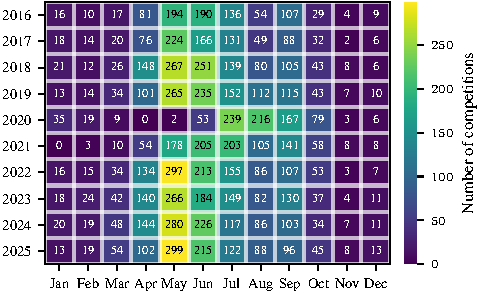
\includegraphics[width=\columnwidth]{figures/COVID_Heatmap_half.pdf}}
\caption{}
\label{covid_heatmap}
\end{center}
\vskip -0.2in
\end{figure}

\begin{figure}[htb]
\vskip 0.2in
\begin{center}
\centerline{
\includegraphics[width=\columnwidth]{figures/covid_relative_performance_change_half_baseline.pdf}}
\caption{}
\label{covid_relative_performance_change}
\end{center}
\vskip -0.2in
\end{figure}
\begin{figure*}[htb]
\vskip 0.2in
\begin{center}
\centerline{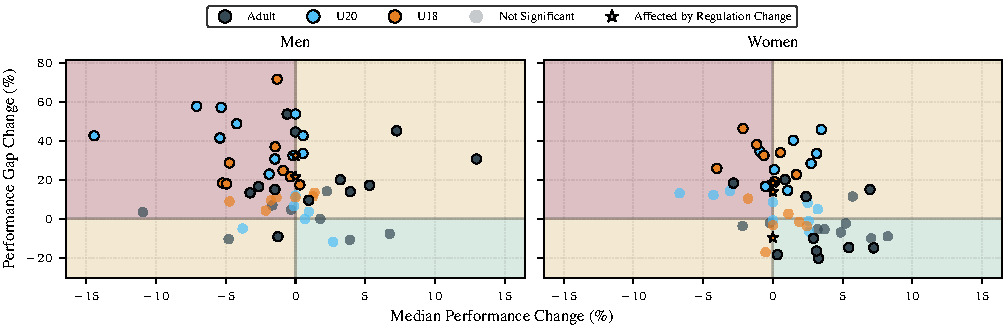
\includegraphics[width=\textwidth]{figures/gap_performance_change.pdf}}
\caption{Change in median performance vs. performance gap (2001–2005 to 2021–2025, in \%) for men and women across age groups. Marker transparency denotes statistical significance for performance gap (p < 0.05). Median changes for disciplines with regulatory updates are fixed at zero due to restricted comparability.
}
\label{gap_perf}
\end{center}
\vskip -0.2in
\end{figure*}

Figure \ref{gap_perf} shows the change in performance spread and typical performance development from 2021-2025 compared to 2001-2005 in many groups. 
The analysis of the performance data encompasses 106 groups, where X groups were excluded for median calculations (see Section \ref{sec:methods}). Overall, a decrease in performance density is evident. The best performers are improving, while the weaker performers are declining.
While median performance trends were nearly balanced with 38 groups significantly improving and 37 declining, the performance spread shows a strong asymmetry: A significant expansion was observed in 49.1\% (52 groups), while a reduction was only seen in 4.7\% (6 groups). This widening of the performance gap was most pronounced among men, especially in the U20 (70.6\%) age group. In contrast, the women's groups showed significantly greater median progress: 63.3\% improved compared to only 36.5\% of the men's groups.
Furthermore, discipline-specific trends emerged: The running and sprinting disciplines showed the most significant progress, with an improvement-to-decline ratio of 3:1 and 2:1 respectively. In contrast, the technical disciplines showed a significant decline: the declines outweighed the improvements by a ratio of 6:1 in throwing and 2.6:1 in jumping.

\begin{figure}[htb]
\vskip 0.2in
\begin{center}
\centerline{
\includegraphics[width=\columnwidth]{figures/rank_performance_change.pdf}}
\caption{Average rank-specific performance development (2001–2005 to 2021-2025, in \%), by age group and sex.}
\label{rank_perf}
\end{center}
\vskip -0.2in
\end{figure}

Figure \ref{rank_perf} illustrates a linear polarization of performance. While the top-ranked company improved by an average of 1.61\%, the 35th-rank declined by 1.51\%, with the turning point towards negative growth being reached at the 22nd-rank. This polarization is not apparent only among adult women; all ranks from third place onward improved more than the top two ranks. Overall, women in all age groups perform better than their male counterparts. The most significant declines were seen in the male age groups under 18 and under 20. In the under-18 age group, the decline begins as early as rank 6, while in the under-20 age group it starts as early as rank 9.

% DISCUSSION
\section{Discussion \& Conclusion}\label{sec:conclusion}
Our results confirm a systematic increase in the performance gap, which aligns with the observed decline in performance at national championships. This reduction in performance density is particularly evident among men and young athletes, where performance differences have widened significantly. A major reason for this structural change is likely the 11.9\% decrease in German Athletics Association (DLV) membership, exacerbated by a 26.6\% drop in the 27- to 60-year-old age group \citep{LeichtathletikPortalDownloads}. Since this age group contains a large number of coaches, its decline directly impacts technical disciplines that rely heavily on expert, individualized training.  In contrast, women’s athletics shows
more improvements, which is probably due to a ”catch-up
effect” as a result of historically delayed professionalization.

Ultimately, the data reveals a polarization of performance: while professionalization protects the national elite, the second tier is shrinking. This confirms our hypothesis that the lack of internal pressure—true to the principle that "competition promotes performance"—has isolated the German elite and ill-prepared them for the intensity of international competition. The zero medal results of recent years are therefore not anomalies, but the predictable outcome of a shrinking talent pool.

In running competitions, the overall improvement in average performance was significantly influenced by the introduction of carbon fiber shoes in 2016 \citep{willwacherDoesAdvancedFootwear2023}. Furthermore, the COVID-19 pandemic led to uneven development. Endurance athletes may benefited from focused, uninterrupted training blocks \citep{venkatesanRunningPerformanceCOVID192022}. In contrast, athletes in technical disciplines were hindered by the closure of training facilities.

One limitation is the focus on the top 35. We cannot make any statements about the general development in all of amateur sports. The analysis only considers advanced competitive sports. Whether the observed trend continues linearly would need to be investigated with further analyses.

The increase in the performance spread indicates a structural change in organized athletics. 
A future focus should be placed on strengthening the grassroots level. 
Following the principle of "the grassroots supporting the elite," this will allow for more top performances and could bring German athletics closer to the world's elite.


% \newpage
\clearpage

\section*{Contribution Statement}
All authors jointly developed the research idea and collaborated closely throughout the project. Maximilian Wernz mainly contributed to data preparation, visualization, and repository management. Erik Müller contributed to data preparation and writing. Mattis Dietrich focused on the performance gap analyses, while Luca Bouché concentrated on the analysis of the COVID-19 pandemic.

% Forces references to align left, removing ugly gaps
{\raggedright
\bibliography{bibliography}
\bibliographystyle{icml2025}
}

\end{document}

% This document was modified from the files available at https://icml.cc/Conferences/2025/AuthorInstructions
% the full copyright notice is available within the file icml2025.sty